\documentclass{proc}
\title{Graphics}
\author{David Corzo}
\date{}

\usepackage{graphicx}
\usepackage[margin=1in]{geometry}


\begin{document}
\maketitle


\section{Let's include some graphics}
Picture books ge the point across \underline{\emph{\textbf{BETTER}}}

\smallskip
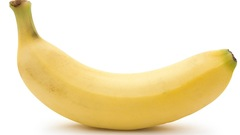
\includegraphics[width=2in]{Banana.jpg}

this is a banana in a jpg

\includegraphics[width=2in]{fish.png}

this is a fish in a png

\subsection{Float: Figure Enviroment}

In my article I want to include a JPG image of a banana. You can see this image in the Figure ~\ref{fig:banana}.

\begin{figure}[htbp]
\begin{center}
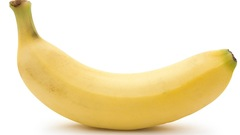
\includegraphics[width=2in]{Banana.jpg}
\caption{This is a banana.}
\label{fig:banana}
\end{center}
\end{figure}

In my article I want to include a PNG image of a chart that look like a fish, you can see this image in Figure ~\ref{fig:fish}

\begin{figure}[htbp]
\begin{center}
\includegraphics[width=2in]{fish.png}
\caption{This is a fish.}
\label{fig:fish}
\end{center}
\end{figure}


\section{}

\section{}



\end{document}





